\documentclass{beamer}
\usepackage[utf8]{inputenc}
\usepackage{datetime2}
\usepackage{multicol}
\usepackage{tikz}
\usepackage{calc}
\usepackage[font=scriptsize]{caption}
\usepackage{csquotes}
\usepackage{xcolor}
\usepackage[ngerman]{babel}
\usetheme{metropolis}
\usepackage[
style=alphabetic,
citestyle=alphabetic,
sorting=nyt]{biblatex}
\addbibresource{literatur.bib}
\setbeamertemplate{frametitle continuation}{\insertcontinuationcount}

% % Definition Progressbar
\makeatletter
\newlength{\custom@progressinheadfoot}
\setbeamertemplate{progress bar in head/foot}{
	\nointerlineskip
	\setlength{\custom@progressinheadfoot}{%
		\paperwidth * \ratio{\insertframenumber pt}{\inserttotalframenumber pt}%
	}%
	\begin{beamercolorbox}[wd=\paperwidth]{progress bar in head/foot}
		\begin{tikzpicture}
		\draw[bg, fill=bg] (0,0) rectangle (\paperwidth, 0.3em);
		\draw[fg, fill=fg] (0,0) rectangle (\custom@progressinheadfoot, 0.3em);
		\end{tikzpicture}%
	\end{beamercolorbox}
}
\addtobeamertemplate{footline}{}{%
	\usebeamertemplate*{progress bar in head/foot}%
}

\tikzset{
    block/.style    = { rectangle, draw=blue, thick, 
	fill=blue!20, text width=6em,
	rounded corners,execute at begin node=\setlength{\baselineskip}{10pt} },
	line/.style     = { draw, thick, ->, shorten >=2pt },
}
{
	\tikzset{terminal/.append style={text height=1.5ex,text depth=.25ex}}
	\tikzset{nonterminal/.append style={text height=1.5ex,text depth=.25ex}}
}

\title{Softwarearchitekturen}
\subtitle{Wie wird ein Entwurf für eine Softwarearchitektur erzeugt?}
\author{Sidney Kuyateh \& Steffen Walter}
\institute{Duale Hochschule Baden-Württemberg}
\date{\today}
\setbeamercolor{progress bar in head/foot}{fg=orange, bg=lightgray}
\begin{document}
	\maketitle
	\begin{frame}[allowframebreaks]{Überblick}
			\tableofcontents[sectionstyle=show, subsectionstyle=show/shaded,]
	\end{frame}
	%%%% Steffen %%%%
		\section{Einführung}
		\metroset{block=fill}
		\subsection{Einführung Softwarearchitekturen}
		\begin{frame}{Einführung Softwarearchitekturen}
			\begin{block}{Definition 1:}
				\enquote{Softwarearchitektur: [...] Strukturierte oder hierarchische Anordnung der Systemkomponenten sowie Beschreibung ihrer Beziehungen.} (\cite{balzert} Seite 520)
			\end{block}
			\begin{block}{Definition 2:}
				\enquote{Strukturen eines Softwaresystems: Softwareteile, die Beziehungen zwischen diesen und die Eigenschaften der Softwareteile und ihrer Beziehungen.} (\cite{clements})
			\end{block}
		\end{frame}
		\section{Architektursichten}
		\subsection{Perspektiven}
			\begin{frame}{Perspektiven}
				\begin{columns}
				\column{0.5\textwidth}
				\begin{itemize}
					\item Es existiert kein Modell, welches alle relevanten Informationen beinhaltet
					\item Verschiedene Perspektiven (vgl. \cite{4+1})
						\begin{itemize}
						\item Logische Sicht
						\item Prozessorientierte Sicht
						\item Entiwicklungsorientierte Sicht
						\item Physische Sicht 
						\textcolor{gray}{\item Konzeptionelle Sicht}
						\end{itemize} 
				\end{itemize}
			   	\column{0.5\textwidth}
			   	\begin{figure}
					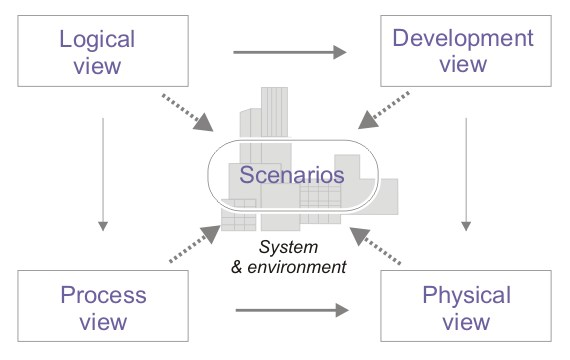
\includegraphics[width=\textwidth]{4+1.jpg}
					\caption{Darstellung 4+1-Sichtenmodell (vgl. \cite{4+1pic})}
				\end{figure}
			\end{columns}
			\end{frame}
			\subsection{Notationen}
			\begin{frame}{Notationen}
			\begin{columns}
			\column{0.5\textwidth}
			\textbf{Informelle Notation (vgl. \cite[ S. 8]{req}}):
				\begin{itemize}
					\item Syntax und Semantik nicht oder nur informell vorgegeben
					\item Beispiel: freie Diagramme
					\item Vorteilhaft bei der Planung und des Entwurfs von Systemarchitekturen (vgl. \cite[ S. 191]{sommer})
				\end{itemize}				
				\column{0.5\textwidth}
				\textbf{Semi-formale Notation (vgl. \cite[ S. 8]{req}}):
				\begin{itemize}
					\item Syntax vorgegeben, Semantik halbformal beschrieben
					\item Beispiele: UML, OCL
					\item Vorteilhaft bei der Dokumentation von Systemarchitekturen (vgl. \cite[ S. 191]{sommer})
				\end{itemize}
			\end{columns}
			\textit{Auch existiert die Architectural Description Language (ADL). Nachteil: sehr spezifisch auf das Anwendungfeld zugeschnitten.}
			\end{frame}
		
		\section{Architekturmuster}
			\subsection{Definition}
			\begin{frame}{Definition}
				\begin{block}{Merkmale von Architekturmustern (vgl. \cite{wulff}):}
					\begin{itemize}
						\item \enquote{Architekturmuster beschreiben die grundsätzliche 
						Struktur und Organisation einer Anwendung und 
						liegen auf der höchsten Abstraktionsebene.}
					
						\item \enquote{Ein Architekturmuster beschreibt die Menge 
						vordefinierter Subsysteme, spezifiziert deren 
						Zuständigkeit und enthält Regeln zu Organisation 
						der Beziehungen zwischen Ihnen.}
					
						\item \enquote{Architekturmuster sind prinzipiell 
						sprach neutral
						und Plattform unabhängig.}
					\end{itemize}
				\end{block}
			\end{frame}
			\subsection{Model-View-Controller-Muster}
			\begin{frame}[allowframebreaks]{Model-View-Controller-Muster}

			   	\begin{figure}
					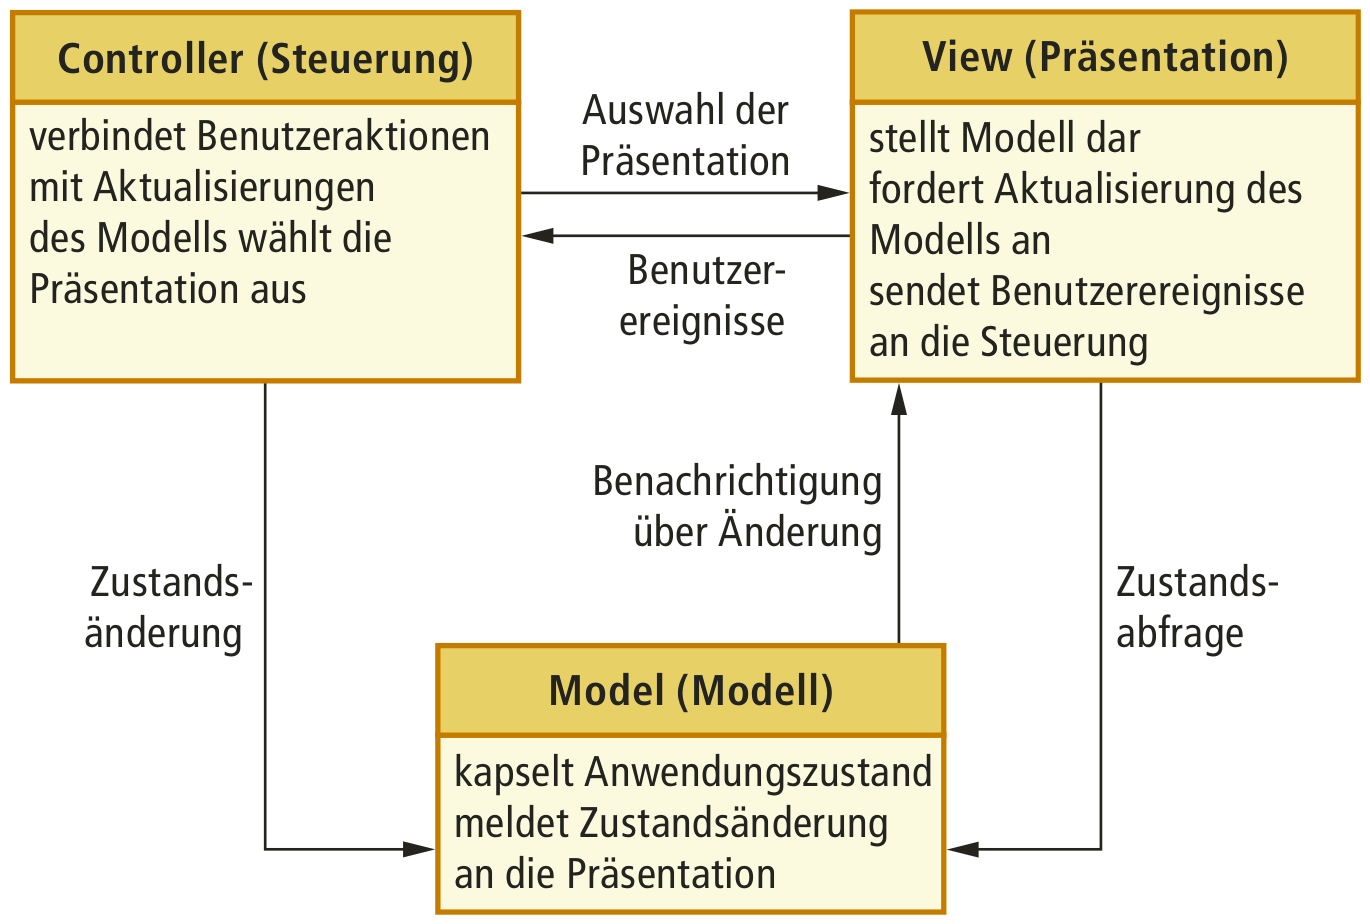
\includegraphics[width=0.8\textwidth]{mvc.png}
					\caption{Model-View-Controller (MVC) (vgl. \cite[ S.193]{sommer})}
				\end{figure}

				\begin{figure}
					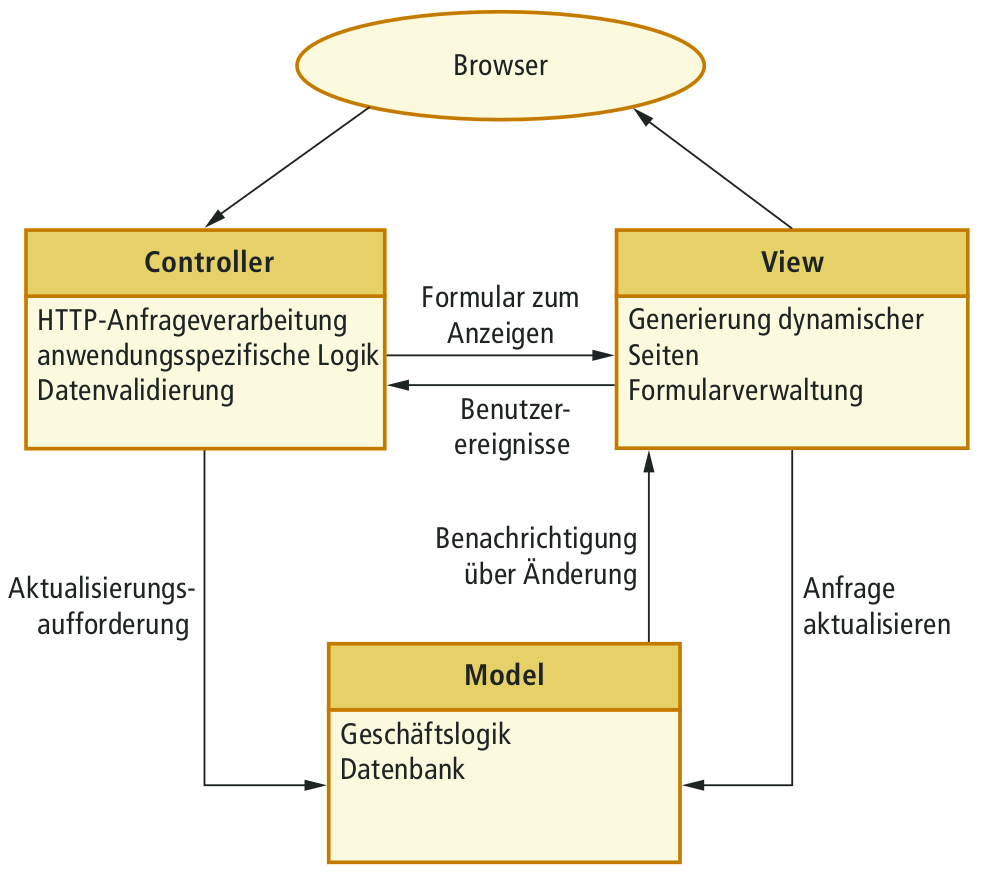
\includegraphics[width=0.65\textwidth]{mvc_bsp.png}
					\caption{Architektur eine Webanwendung im MVC-Modell (vgl. \cite[ S.193]{sommer})}
				\end{figure}
			\end{frame}
			\subsection{Schichtenarchitektur}
			\begin{frame}{Schichtenarchitektur}
			
			\end{frame}
			\subsection{Repository-Architektur}
			\begin{frame}{Repository-Architektur}
			
			\end{frame}	
			\subsection{Client-Server-Architektur}
			\begin{frame}{Client-Server-Architektur}
			
			\end{frame}
			\subsection{Pipes-and-Filter-Architektur}
			\begin{frame}{Pipes-and-Filter-Architektur}
			
			\end{frame}	
	%%%% Sidney %%%%
	\section{Anwendungsarchitekturen}
		\subsection{Nutzung von Anwendungsarchitekturen}
			\begin{frame}{Nutzung von Anwendungsarchitekturen}
				\begin{itemize} % sommer
					\item Enthalten die Haupteigenschaften einer Systemklasse
					\item Allgemeine architektonische Struktur kann beibehalten werden für neue Systeme desselben Typs
					\item
				\end{itemize}
			\end{frame}
		\subsection{Transaktionsverarbeitende Systeme}
			\begin{frame}{Transaktionsverarbeitende Systeme}
				\begin{block}{Definition:}
					\enquote{Das Ziel Transaktionsverarbeitender Systeme (TP) ist die Verarbeitung von Benutzeranfragen nach Informationen aus einer Datenbank oder Anfragen zum Aktualisieren der Datenbank.} \cite[S. 204]{sommer}
				\end{block}
				\begin{itemize}
					\item Alle Schritte der Transaktion müssen abgeschlossen sein, bevor Änderungen in die Datenbank geschrieben werden
					\item Transaktionsmanager ist für die Kommunikation mit der Datenbank verantwortlich
				\end{itemize}
				\begin{figure}
					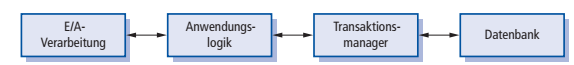
\includegraphics[width=\textwidth]{transaktionssystem-1.png}
					\caption{Die Struktur transaktionsverarbeitender Anwendungen \cite[S. 204]{sommer}}
				\end{figure}
			\end{frame}
		\subsection{Informationssysteme}
			\begin{frame}{Informationssysteme 1}
			\begin{itemize}
				\item Alle Systeme mit einer gemeinsam genutzten Datenbank können als transaktionsbasierte Informationssysteme betrachtet werden (vgl. \cite[S. 205]{sommer})
				\item Kontrollierter Zugriff auf eine große Informationsbasis
			\end{itemize}
			\begin{figure}
				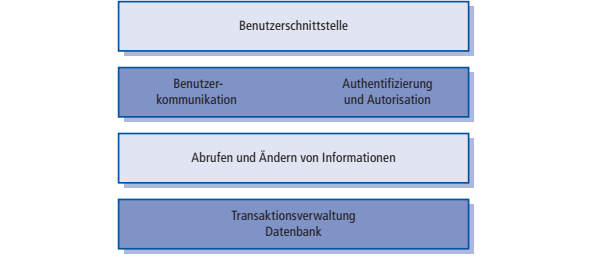
\includegraphics[width=\textwidth]{informationssystem-1.png}
				\caption{Schichtenarchitektur eines Informationssystems \cite[S. 205]{sommer}}
			\end{figure}
			\end{frame}
		
			\begin{frame}{Informationssysteme 2}
			\begin{itemize}
				\item Heutzutage meist webbasierte Systeme
				\item Schichten häufig softwaretechnisch aufgeteilt:
				\begin{itemize}
					\item Webserver: Benutzerkommunikation
					\item Anwendungsserver: Anwendungslogik, Abrufen und Ändern von Informationen
					\item Datenbankserver: Transaktionsmanagement, Ausführen der Datenbankoperationen
				\end{itemize}
			\end{itemize}
			\end{frame}
			
		\subsection{Sprachverarbeitende Systeme}
			\begin{frame}{Sprachverarbeitende Systeme}
				\begin{itemize}
					\item Übersetzen eine natürliche oder künstliche Sprache in eine andere Darstellung \cite[S. 207]{sommer}
					\item Beispiele: Compiler, Dateikonverter, Natürliche Übersetzungssysteme
				\end{itemize}
			\begin{figure}
				\begin{tikzpicture}
				\matrix[ampersand replacement=\&, column sep = 5mm, row sep = 5mm] {
					\node (p1) [block] {\tiny Anweisungen der Quellsprache}; \& \node (p2) [block] {\tiny Übersetzer: \\ Syntax prüfen; \\ Semantik prüfen; \\ Erstellen}; \& \\
					\& \node (p3)  [block]  {\tiny abstrakte Maschinenanweisungen}; \& \\
					\node (p4) [block] {\tiny Daten}; \& \node (p5) [block] {\tiny Interpreter: \\ abrufen; \\ ausführen}; \&
					\node (p6) [block]  {\tiny Ergebnisse};\\
				};
				\end{tikzpicture}
				\caption{text}
			\end{figure}
			
				
			%	\begin{figure}
			%		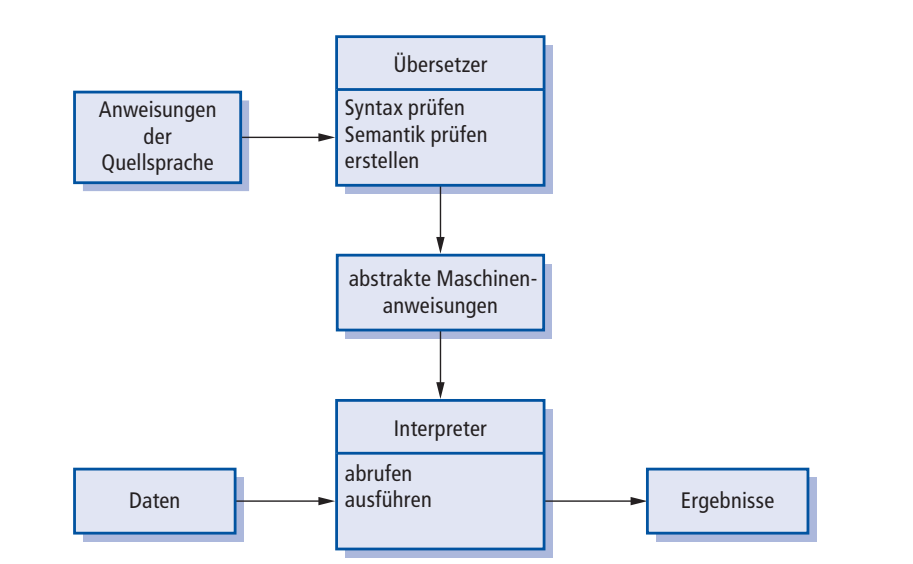
\includegraphics[width=0.7\textwidth]{sprachsystem-1.png}
			%		\caption{text}
			%	\end{figure}
			\end{frame}
	\begin{frame}[allowframebreaks]
		\frametitle{Quellen}
		\printbibliography[heading=none]
	\end{frame}
\end{document}


